%!TEX root = ../../../FYP_Dissertation.tex

This module is a simple command line interface to the built-in
low-overhead profiler of LuaJIT. The lower-level API of the profiler
is accessible via the "jit.profile" module or the LuaJIT\_profile\_* C API.

Example usage:
\begin{lstlisting}
  mad -jp myapp.mad
  mad -jp=s myapp.mad
  mad -jp=-s myapp.mad
  mad -jp=vl myapp.mad
  mad -jp=G,profile.txt myapp.mad
\end{lstlisting}
The following dump features are available:
 \begin{itemize}%[label={--}]
  \item \textbf{f} - Shows function name (Default mode).
  \item \textbf{F} - Shows function name with module prepend.
  \item \textbf{l} - Shows line granularity ('module':'line').
  \item \textbf{\textless number\textgreater} - Stack dump depth (callee\textless caller - Default: 1)
  \item \textbf{-\textless number\textgreater} - Inverse stack dump depth (caller\textgreater callee).
  \item \textbf{s} - Split stack dump after first stack level. Implies $\mid depth\mid$
  \textgreater= 2.
  \item \textbf{p} - Show full path for module names.
  \item \textbf{v} - Show VM states (See bellow).
  \item \textbf{z} - Show zones (See bellow).
  \item \textbf{r} - Show raw sample counts (Default: percentages).
  \item \textbf{a} - Annotate excerpts from source code files.
  \item \textbf{A} - Annotate complete source code files.
  \item \textbf{G} - Produce raw output suitable for graphical tools (See bellow).
  \item \textbf{m\textless number\textgreater} - Minimum sample percentage to be shown (Default: 3).
  \item \textbf{i\textless number\textgreater} - Sampling interval in milliseconds (Default: 10).
 \end{itemize}

 Many of those options can be activated at ones.\\

We can also use this module programmatically like in the example below. The
\emph{start} function can take 2 arguments, the list of options (describe above)
and the output file.
\begin{lstlisting}[style=LuaStyle]
local prof = require"jit.p"
prof.start("vf", "file.txt")
  -- Code to analyze here
prof.stop()
\end{lstlisting}

\paratitle{VM states:}\\
This option allows to shows the time spent in which state of the VM.
States can be of the following types :

\{Compiled - Interpreted - C code - Garbage Collector - JIT Compiler\} \\

\paratitle{Zone:}\\
Statistics can be grouped in user defined zone. Below is an example a such a
definition.
\begin{lstlisting}
    local zone = require("jit.zone")
    zone("MyZone")
      -- Lua code here
    zone()
\end{lstlisting}

\paratitle{Graphical tools:}\\
This option can be used to graphically show the dump in a nice image format
(see Appendix \ref{Apendix:fl})

Figure \ref{fig:profiler} shows two different output of the run of the
\emph{Sequence} tests presented in Part \ref{Part:mad}. On the left we can see
the default mode of the profiler with the percentage of time spent per function.
On the right we see the percentage of time spent per VM states (the \emph{v} mode).

\begin{figure}[H]
    \centering
    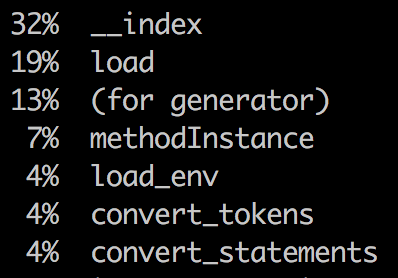
\includegraphics[height=3.5cm]{./Images/profiler-1}
    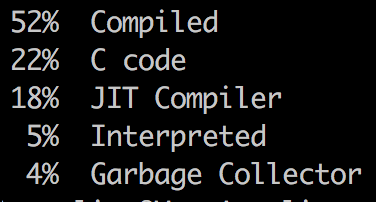
\includegraphics[height=3.5cm]{./Images/profiler-2}
    \caption{Screenshot of the profiler output}
    \label{fig:profiler}
\end{figure}
